% !TeX root=../main.tex
\chapter{نتایج}
%\thispagestyle{empty} 
\label{chap:results}
\section{مقدمه} \label{introduction}
در این بخش به ارزیابی نتایج بدست آمده از الگوریتم پیشنهادی پرداخته می‌شود. بخش %
\ref{datasets}
مجموعه داده‌ های استفاده شده را شامل می‌شود. بخش %
\ref{meyar_shive_piyade}
معیار‌ها و شیوه‌های ارزیابی مرتبط با تحقیق، توضیح داده شده است. در بخش %
\ref{zojiyate_piyade}
جزییات پیاده سازی، سیستم استفاده شده و یک سری تنظیمات مربوط به مدل توضیح داده شده است.
 در بخش‌های %
\ref{natayej_majmoe_dade}
و
\ref{natayej_majmoe_dade2}
نتایج آزمایش روی مجموعه داده‌های مختلف و دو الگوریتم پیشنهادی گزارش شده است. و درنهایت بخش %
\ref{amig_negah}
یک نگاه کوتاه به خروجی مدل و نحوه نگاه مدل به مسئله بررسی شده است.

\section{‌معرفی مجموعه داده‌ها} \label{datasets}
داده های این پایان نامه، تصاویر مربوط به فعالیت های مختلف از دو مجموعه داده %
\lr{Stanford40}
 و %
 \lr{Pascal VOC‌ 2012}
 می‌باشد که اغلب کارها این دو مجموعه داده در فرآیند آموزش و ارزیابی مورد استفاده قرار می‌گیرد.
 
\lr{\textbf{ Stanford40}}
: این مجموعه داده یکی از شناخته شده ترین مجموعه داده های موجود در زمینه تشخیص فعالیت انسان در تک تصویر می‌باشد که شامل 40 کلاس از دسته بندی‌های مختلف مانند حرکات ورزشی، بازی‌ها و یک سری فعالیت های روزانه است. این مجموعه داده 4000 تصویر برای آموزش و 5530 تصویر برای ارزیابی دارد.
 
 \lr{\textbf{ Pascal VOC‌ 2012 }}
 : این مجموعه داده شامل 4588 تصویر برای 10 تا دسته بندی دارد که از این تعداد 2296 تصویر را در بخش آموزش و 2292 تصویر در بخش ارزیابی قرار دارد. درحالی که تعداد کلاس‌های این مجموعه داده کمتر از قبلی است اما چالش بیشتری نسبت به مجموعه داده قبلی دارد و تصاویر از کیفیت پایین‌تری برخوردار است. همچنین دریک تصویر ممکن است که چند شخص با فعالیت های مختلف قرار داشته باشد که این یک چالش اساسی است.
 
 دربین این دوتا مجموعه داده، %
 \lr{Stanford40}
 بیشتر از %
 \lr{Pascal VOC}
 مورد استفاده قرار می‌گیرد. هردوی این مجموعه داده‌ها نواحی انسان را مشخص کرده اند و ناحیه‌ی اشیاء از کدهای منتشر شده کار%
 \cite{Human_object_relation_action}
 قابل استفاده است.
 
 \section{‌معیار و شیوه‌های ارزیابی} \label{meyar_shive_piyade}
 در مسائل مختلف معیارهاي ارزیابی متفاوتی استفاده می‌شود، اما برخی معیارهاي ارزیابی به دلیل استاندارد بودن در بسیاري پژوهش‌ها مورد استفاده قرار می‌گیرند. در این پایان نامه نیز سعی شده است تا الگوریتم پیشنهادي با برخی از این معیارهای کمی مورد ارزیابی قرار گیرد.
 
 برای استفاده از معیار‌های کمی ارزیابی،‌ دوحالت را برای فعالیت انسان در نظر می‌گیریم،‌ یا فعالیت بدست آمده مربوط با تصویر است یا نامرتبط با آن است. اگر مرتبط باشد و بیانگر همان فعالیت درحال انجام باشد، مثبت و اگر فعالیتی وجود نداشته باشد، منفی درنظر گرفته می‌شود.
 
\textbf{مثبت درست}
 \LTRfootnote{True Positive}
 : زمانی رخ می‌دهد که مدل فعالیتی را درتصویر تشخیص می‌دهد که در برچسب نیز همان فعالیت است و نشان می‌دهد که فعالیت در تصویر و برچسب یکسان است.
 
\textbf{مثبت غلط}
\LTRfootnote{False Positive}
: زمانی رخ می‌دهد که مدل فعالیتی را در تصویر تشخیص می‌دهد اما در مجموعه داده‌های ما فعالیتی برای آن تعریف نشده یا وجود ندارد.

\textbf{منفی درست}
\LTRfootnote{True Negative}
: زمانی رخ می‌دهد که مدل عدم وجود فعالیت را تشخیص می‌دهد و برچسب یا مجموعه داده اصلی مانیز عدم حضور فعالیت را نشان می‌دهد.

  \textbf{منفی غلط}
  \LTRfootnote{False Negative}
  : زمانی رخ می‌دهد که مدل عدم وجود فعالیت را تشخیص می‌دهد اما برچسب وجود فعالیت را نشان می‌دهد.
  
  \textbf{\gls{Accuracy}}
  : یکی از معیارهای ارزیابی متداول برای اندازه‌گیری عملکرد یک مدل طبقه‌بندی است. این معیار نسبت تعداد نمونه‌هایی که به درستی طبقه‌بندی شده‌اند (هم پیش‌بینی‌های مثبت و هم پیش‌بینی‌های منفی) به تعداد کل نمونه‌ها را نشان می‌دهد.
\begin{equation}
	\text { Accuracy }=\frac{T P+T N}{T P+T N+F P+F N}
\end{equation}
\textbf{\gls{Precision}}
 : تعداد نمونه‌هایی که از یک کلاس خاص به درستی تشخیص داده شده‌اند، نسبت به تعداد کل نمونه‌هایی که به اشتباه به آن کلاس اختصاص داده شده‌اند.
  \begin{equation}
  	\text { Precision }=\frac{T P}{T P+F P}
  \end{equation}
  \textbf{\gls{Recall}}
 : یکی از معیارهای ارزیابی عملکرد مدل‌های دسته‌بندی است که نسبت تعداد نمونه‌های مثبتی را که به درستی تشخیص داده شده‌اند به تعداد کل نمونه‌های مثبت در داده‌های آزمون را نشان می‌دهد.
  \begin{equation}
  	\text { Recall }=\frac{T P}{T P+F N}
  \end{equation}
    \textbf{میانگین متوسط دقت}
  \LTRfootnote{Mean Average Precision}
: در مسائل تشخیص فعالیت انسان در تک تصویر، معیار mAP به منظور ارزیابی عملکرد مدل‌های دسته‌بندی استفاده می‌شود. این معیار از AP%
 \LTRfootnote{Average Precision}
 ها برای هر کلاس محاسبه می‌شود و سپس میانگین آن‌ها برای تمام کلاس‌ها گرفته می‌شود. mAP نشان می‌دهد که مدل در تشخیص فعالیت مختلف در تصاویر چقدر موفق بوده است.
 \begin{equation}
 	\mathrm{mAP}=\frac{1}{N} \sum_{i=1}^N \mathrm{AP}_i
 \end{equation}
     \textbf{\gls{ConfusionMatrix}}
: ماتریس درهم ریختگی یک ابزار ارزیابی است که برای اندازه‌گیری عملکرد مدل‌های دسته‌بندی استفاده می‌شود. این ماتریس برای مدل‌هایی که به صورت دودویی (با دو کلاس مثبت و منفی) طبقه‌بندی می‌کنند، به کار می‌رود. اما می‌توان آن را برای مسائل با چند کلاس نیز گسترش داد. شکل %
\ref{fig:confution_matrix_explain}
نحوه چینش ماتریس درهم ریختگی را نشان می‌دهد. البته طول ماتریس ممکن است متفاوت باشد اما همچنان این نوع ساختار درآن حفظ می‌شود.
\begin{figure}[ht]
	\centerline{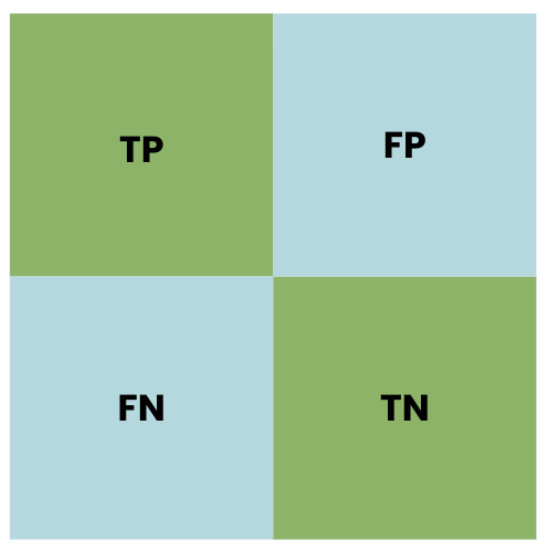
\includegraphics[width=0.2\textwidth]{confution_matrix_explain}}
	\caption{نمونه ماتریس درهم ریختگی}
	\label{fig:confution_matrix_explain}
\end{figure}
\vspace{-10pt}
 \section{‌جزئیات پیاده سازی}\label{zojiyate_piyade}
تمامی آزمایشات این پایان نامه با زبان پایتون کدنویسی شده و در سیستم عامل لینوکس اوبونتو و روی کامپیوتر با مشخصات حافظه داخلی 16 گیگابایت و گرافیک 4 گیگابایت تست شده است. آموزش های مدل روی سیستم مجازی %
\lr{Google Colab}
انجام شده است که این سیستم گرافیک تا 14 گیگابایت را در اختیارمان قرار داد. الگوریتم معرفی شده در چارچوب MXNet پیاده سازی شده است.\\
درمرحله آموزش %
\lr{Loss Function} 
که استفاده شده %
\lr{Cross-Entropy}
است و بهینه ساز مورد نظر نیز‌ %
\gls{StochasticGradientDescent}
انتخاب شده است. نرخ یادگیری را %
\rl{4e-4}
 ،  %
 \gls{Momentum}
 9.0
 و تعداد حلقه های آموزش 15 درنظر گرفته شده است. همچنین نرخ آموزش در این 15 تکرار از $3*10^{-5}$ به $1*10^{-6}$ کاهش می‌یابد.\\
در بخش بدنه اصلی مدل از %
\lr{ResNet50}
استفاده شده است که فرآیند استخراج ویژگی را انجام می‌دهد. نقاط کلیدی بدن انسان نیز با دو الگوریتم yolo و mmpose استخراج شده است.
 \section{نتایج روی مجموعه داده ‌های  \lr{Stanford40}} \label{natayej_majmoe_dade}
 ارزیابی نتایج دو الگوریتم پیشنهادی در جدول %
 \ref{tab:jadval_degat_all}
 نشان داده شده است.
 \begin{table}[h!]
 	\centering
	\begin{tabularx}{0.8\textwidth} { 
			  >{\raggedleft\arraybackslash}X 
			 >{\raggedleft\arraybackslash}X 
			 p{2cm} >{\raggedleft\arraybackslash}X  }
		\hline
 \textbf{الگوریتم} & \textbf{بدنه اصلی} & \textbf{میانگین دقت (mAP)}\\
		\hline
		Attention %
		\cite{Multi_branch_Attention_Recg_still}
		& \lr{VGG 16} & \lr{90.7} \\
		R*CNN %
		\cite{contextual_action_rcnn}
		& \lr{VGG 16} & \lr{90.9} \\
		Part Action %
		\cite{Single_image_semantic_body}
		& \lr{ResNet-50} & \lr{91.2} \\
		Loss Guided %
		\cite{Loss_guided_actv_attention}
		& \lr{ResNet-50} & \lr{91.1} \\
		KPs-Assisted %
		\cite{a_key_points_assisted_net}
		& \lr{EfficientNetV2} & \lr{91.8} \\
		Relation %
		\cite{Human_object_relation_action}
		& \lr{ResNet-50} & \lr{\textbf{93.1}} \\
		\hline
		روش پیشنهادی + ارتباط‌سنج
		& \lr{ResNet-50} & \lr{\textbf{92.6}} \\
		روش پیشنهادی + LAD
		& \lr{ResNet-50} & \lr{\textbf{92.7}} \\
		\hline
	\end{tabularx}
	\caption{دقت روش‌های مختلف روی مجموعه داده \lr{Stanford40}}
	\label{tab:jadval_degat_all}
\end{table}
همانطورکه آزمایش شد،‌ استفاده از ژست در این مجموعه داده منجربه دقت پایین تری نسبت به روش %
\cite{Human_object_relation_action}
شد. همچنین نبود وزن‌های‌ اولیه آماده در مدل های قبلی و مدل پیشنهادی کار آموزش مدل‌ها با کندی پیش رفت که صرف هزینه زمانی زیادی شد. البته از بدنه قوی تری نیز استفاده نشد زیرا مدل‌های قبلی از این بدنه برای ارزیابی استفاده کردند و ما نیز از این بدنه استفاده کردیم که دریک شرایط برابر مقایسه انجام شود.
با این حال استفاده از ژست مخصوصا اضافه کردن بردار ویژگی بهبود یافته توصیف کننده زاویه بدن%
\LTRfootnote{iLAD}
 یک مقدار عملکرد بهتری نسبت به روش ارتباط‌سنج گزارش داد.
 
 ماتریس درهم‌ریختگی یک ابزار مفید در ارزیابی نتایج می‌باشد. شکل %
\ref{fig: confution_matrix_std_m}
ماتریس درهم‌ریختگی روش پیشنهادی با ارتباط‌سنج نشان می‌دهد.
  \begin{figure}[ht]
  	\centerline{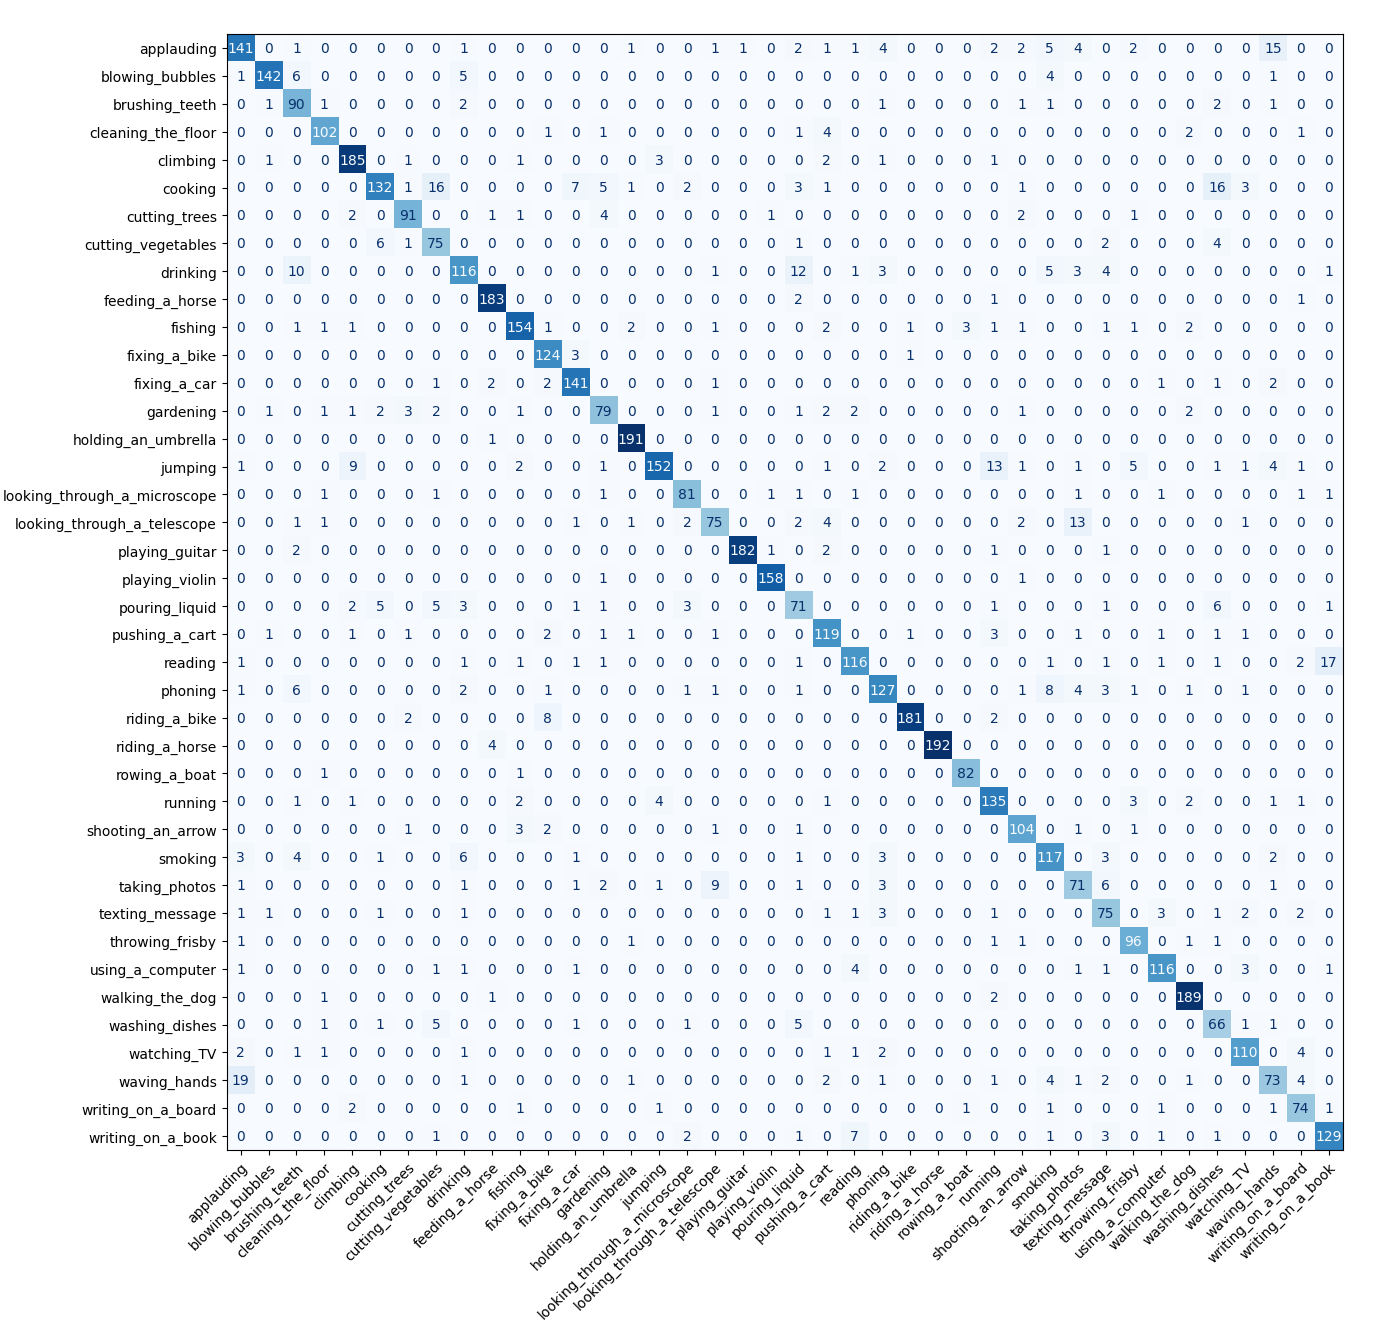
\includegraphics[width=0.9\textwidth]{confution_matrix_std40}}
  	\caption{ماتریس درهم ریختگی روش ارتباط‌سنج روی \lr{Stanford40}}
  	\label{fig: confution_matrix_std_m}
  \end{figure}
  
  طبق این نتایج بدست آمده، فعالیت "تشویق کردن" با 15 دسته‌بندی اشتباه و "تکان دادن دست" با 19 اشتباه جزء فعالیت‌های دشوار برای این مدل به شمار می‌روند. علت این دسته‌بندی نادرست نزدیک بودن دو فعالیت در حالت دست ها است. به دلیل نبودن اطلاعات زمانی و حرکتی مدل نمی‌تواند تفکیک درستی از حرکت دست ‌ها و تخمین فعالیت داشته باشد.\\
همچنین فعالیت "آشپزی کردن" با 16 دسته‌بندی نادرست از کلاس "شستن ظرف" نشان می‌دهد که وجود ظرف درهر دو فعالیت باعث گمراهی ‌مدل شده است. دراینجا نیز نبود اطلاعات حرکتی عامل اصلی این دسته‌بندی نادرست است.

  در شکل %
  \ref{fig: confution_matrix_std40_lad}
   ماتریس درهم‌ریختگی برای روش توصیف کننده زاویه بدن نشان داده شده است.
    \begin{figure}[ht]
  	\centerline{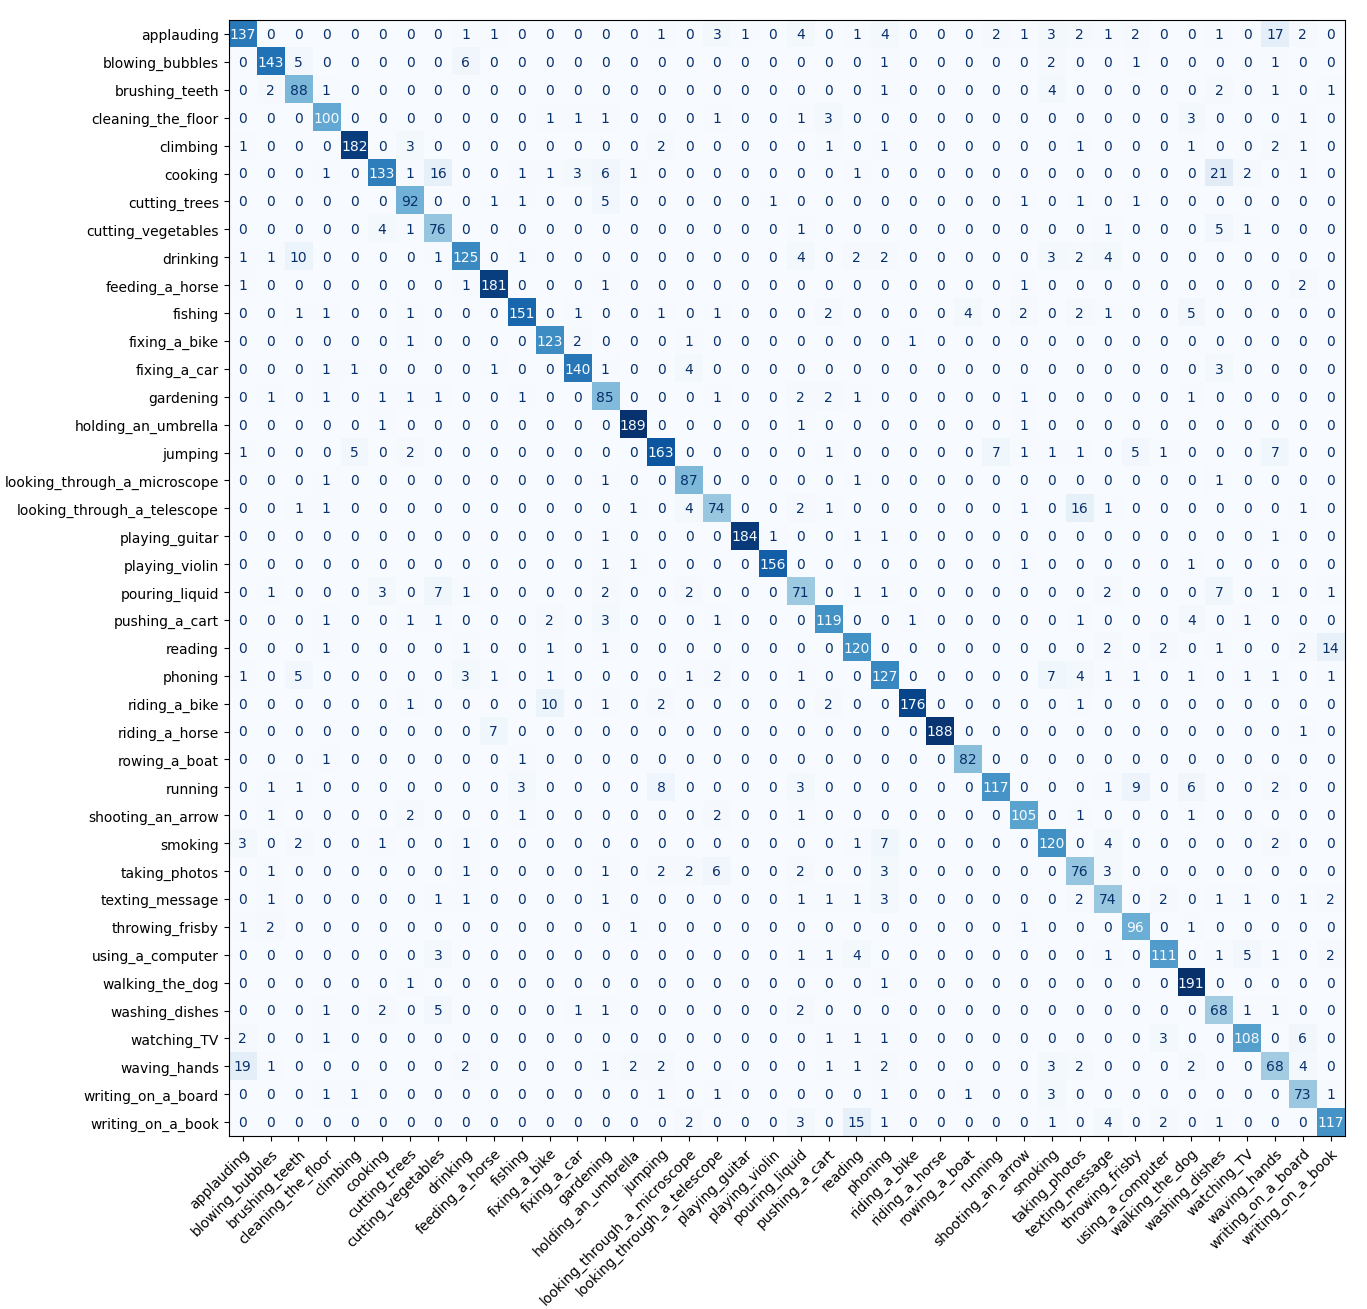
\includegraphics[width=0.9\textwidth]{confution_matrix_std40_lad}}
  	\caption{ماتریس درهم ریختگی روش توصیف کننده زاویه بدن روی \lr{Stanford40}}
  	\label{fig: confution_matrix_std40_lad}
  \end{figure}
  همانطور که در شکل مشخص است، بیشتری دسته بندی نادرست مربوط به فعالیت "آشپزی کردن" است که 21 تصویر از فعالیت "شستن ظرف" را به اشتباه فعالیت "آشپزی کردن" پیش بینی کرده است. این نشان می‌دهد که فعالیت های "آشپزی کردن" و "شستن ظرف" جزء سخت ترین فعالیت‌ ها در این مجموعه داده است.
دو فعالیت "اسب سواری" و "ویالون زدن" جز دوتا فعالیتی هستند که کمترین خطا را داشتند و هر دو مدل به درستی توانسته‌‌اند این دو را دسته بندی کنند.
 \begin{table}[h!]
	\centering
	\fontsize{10pt}{10pt}\selectfont
	\begin{tabularx}{0.8\textwidth} { 
			| >{\raggedleft\arraybackslash}X 
			| >{\raggedleft\arraybackslash}X 
			| >{\raggedleft\arraybackslash}X
			| >{\raggedleft\arraybackslash}X |
			 }
		\hline
		\textbf{بیشترین ها} & \textbf{دقت (\%)} & \textbf{کمترین ها} & \textbf{دقت (\%)} 
		\\
		\hline
		اسب سواری &
		\lr{99.9} &
		تکان دادن دست &
		\lr{73.2}\\
		\hline
		ویالون زدن &
		\lr{99.9} &
		سرریز کردن آب &
		\lr{79.5} \\
		\hline
		گیتار زدن &
		\lr{99.8} &
		عکس گرفتن &
		\lr{81.0} \\
		\hline
	\end{tabularx}
	\caption{ سه تا از بیشترین و کمترین دقت ها روی \lr{Stanford40}}
	\label{tab:jadval_degat_best_std}
\end{table}
\section{نتایج روی مجموعه داده‌ های \lr{VOC 2012}}\label{natayej_majmoe_dade2}
این مجموعه داده چالش بیشتری نسبت به مجموعه داده %
\lr{Stanford40}
 دارد. نتایج ارزیابی روی این مجموعه داده در جدول %
  \ref{tab:jadval_degat_all_voc}
  نشان داده شده است.
  \begin{table}[h!]
  	\centering
  	\fontsize{10pt}{10pt}\selectfont
  	\begin{tabularx}{0.99\textwidth} { 
  			p{2.3cm}>{\raggedleft\arraybackslash}X 
  			>{\raggedleft\arraybackslash}X 
  			>{\raggedleft\arraybackslash}X 
  			>{\raggedleft\arraybackslash}X 
  			>{\raggedleft\arraybackslash}X 
  			>{\raggedleft\arraybackslash}X 
  			>{\raggedleft\arraybackslash}X 
  			>{\raggedleft\arraybackslash}X 
  			>{\raggedleft\arraybackslash}X 
  			>{\raggedleft\arraybackslash}X 
  			| >{\raggedleft\arraybackslash}X 
  			>{\raggedleft\arraybackslash}X  }
  		\hline
  		\textbf{الگوریتم} & \textbf{پریدن} & \textbf{تلفن زدن} & \textbf{ساز زدن} & \textbf{خواندن} & \textbf{دوچرخه سواری} & \textbf{اسب سواری} & \textbf{دویدن} & \textbf{عکس گرفتن} & \textbf{استفاده کامپیوتر} & \textbf{راه رفتن} & \textbf{دقت}
  		\\
  		\hline
  		Attention %
  		\cite{Multi_branch_Attention_Recg_still}
  		& \lr{87.8} & \lr{78.4} & \lr{93.7} & \lr{81.1} & \lr{95.0} & \lr{97.1} & \lr{\textbf{96.0}} & \lr{85.5} & \lr{93.1} & \lr{73.4} & \lr{87.1}
  		\\
  		R*CNN %
  		\cite{contextual_action_rcnn}
  		& \lr{88.9} & \lr{79.9} & \lr{95.1} & \lr{82.2} & \lr{96.1} & \lr{97.8} & \lr{87.9} & \lr{85.3} & \lr{94.0} & \lr{71.5} & \lr{87.9}\\
  		Part Action %
  		\cite{Single_image_semantic_body}
  		& \lr{89.6} & \lr{86.9} & \lr{94.4} & \lr{\textbf{88.5}} & \lr{94.9} & \lr{97.9} & \lr{91.3} & \lr{87.5} & \lr{92.4} & \lr{76.4} & \lr{90.0} \\
  		Relation %
  		\cite{Human_object_relation_action}
  		& \lr{89.2} & \lr{89.8} & \lr{96.5} & \lr{87.6} & \lr{\textbf{98.2}} & \lr{99.1} & \lr{92.3} & \lr{91.6} & \lr{95.2} & \lr{79.2} & \lr{91.9} \\
  		Patch %
  		\cite{patch_boxless_action}
  		& \lr{89.0} & \lr{86.6} & \lr{95.0} & \lr{87.7} & \lr{95.7} & \lr{96.7} & \lr{92.3} & \lr{82.0} & \lr{95.6} & \lr{72.7} & \lr{89.3} \\
  		\hline
پیشنهادی(ارتباط‌سنج)
  		& \lr{90.7} & \lr{89.3} & \lr{95.6} & \lr{86.7} & \lr{97.7} & \lr{98.8} & \lr{93.2} & \lr{90.5} & \lr{\textbf{95.6}} & \lr{\textbf{80.2}} & \lr{91.9} \\
  		پیشنهادی(LAD)
  		& \lr{\textbf{91.5}} & \lr{\textbf{90.9}} & \lr{\textbf{97.0}} & \lr{87.4} & \lr{97.5} & \lr{\textbf{99.1}} & \lr{93.1} & \lr{\textbf{92.5}} & \lr{95.1} & \lr{78.9} & \lr{\textbf{92.33}} \\
  		\hline
  	\end{tabularx}
  	\caption{دقت روش‌های مختلف روی مجموعه داده \lr{VOC 2012}}
  	\label{tab:jadval_degat_all_voc}
  \end{table}
 همانطور که طبق جدول %
  \ref{tab:jadval_degat_all_voc}
  مشاهده می‌کنید، روش پیشنهادی توصیف کننده زاویه بدن روی این مجموعه داده عملکرد بسیاری خوبی از خود نشان داده است. در فعالیت های "پریدن" ، "تلفن زدن" ، "ساز زدن" ، "اسب سواری" ، "عکس گرفتن" بیشترین دقت ها را بین رقبای خود بدست آورده است و میانگین متوسط دقت 33.92\% بیشترین دقت در این بین می‌باشد.
  
  در تصویر %
\ref{fig: confiution_matrixvoc}
و 
\ref{fig: confution_matrix_voclad}
ماتریس درهم‌ریختگی برای روش ارتباط‌سنج و توصیف کننده زاویه بدن نشان داده شده است. در این دو تصویر دو فعالیت "دویدن" و "راه رفتن" چندین نمونه دسته‌بندی اشتباه داشتند. دلیل اصلی این اشتباهات نیز نبود را می‌توان نبود اطلاعات حرکتی و زمانی در تک تصویر معنا کرد. زیر مرز باریکی بین دویدن و راه رفتن در تصویر وجود دارد. دسته "موارد دیگر" به دلیل مشخص نبودن نوع فعالیت و تصاویر به هم ریخته و نامنظم نادیده گرفته می‌شود. \\
نمودار %
\ref{fig: nemodar_natije_relation_pish}
تفاوت بین روش پیشنهادی با توصیف کننده زاویه بدن و مقاله %
\cite{Human_object_relation_action}
را نشان می‌دهد.

\begin{figure}[ht]
	\centerline{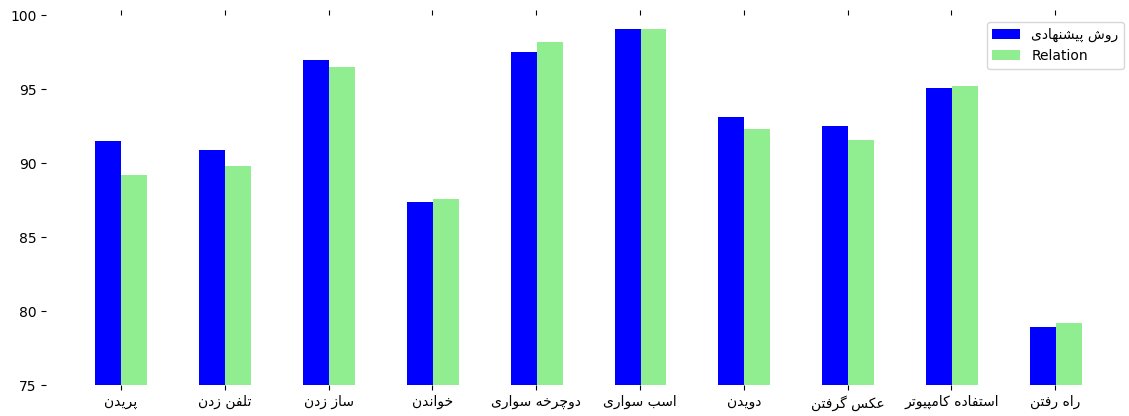
\includegraphics[width=0.9\textwidth]{nemodar_r_p}}
	\caption{نمودار مقایسه نتایج روش پیشنهادی توصیف کننده بدن با \lr{Relation}}
	\label{fig: nemodar_natije_relation_pish}
\end{figure}
\begin{figure}[ht]
	\centerline{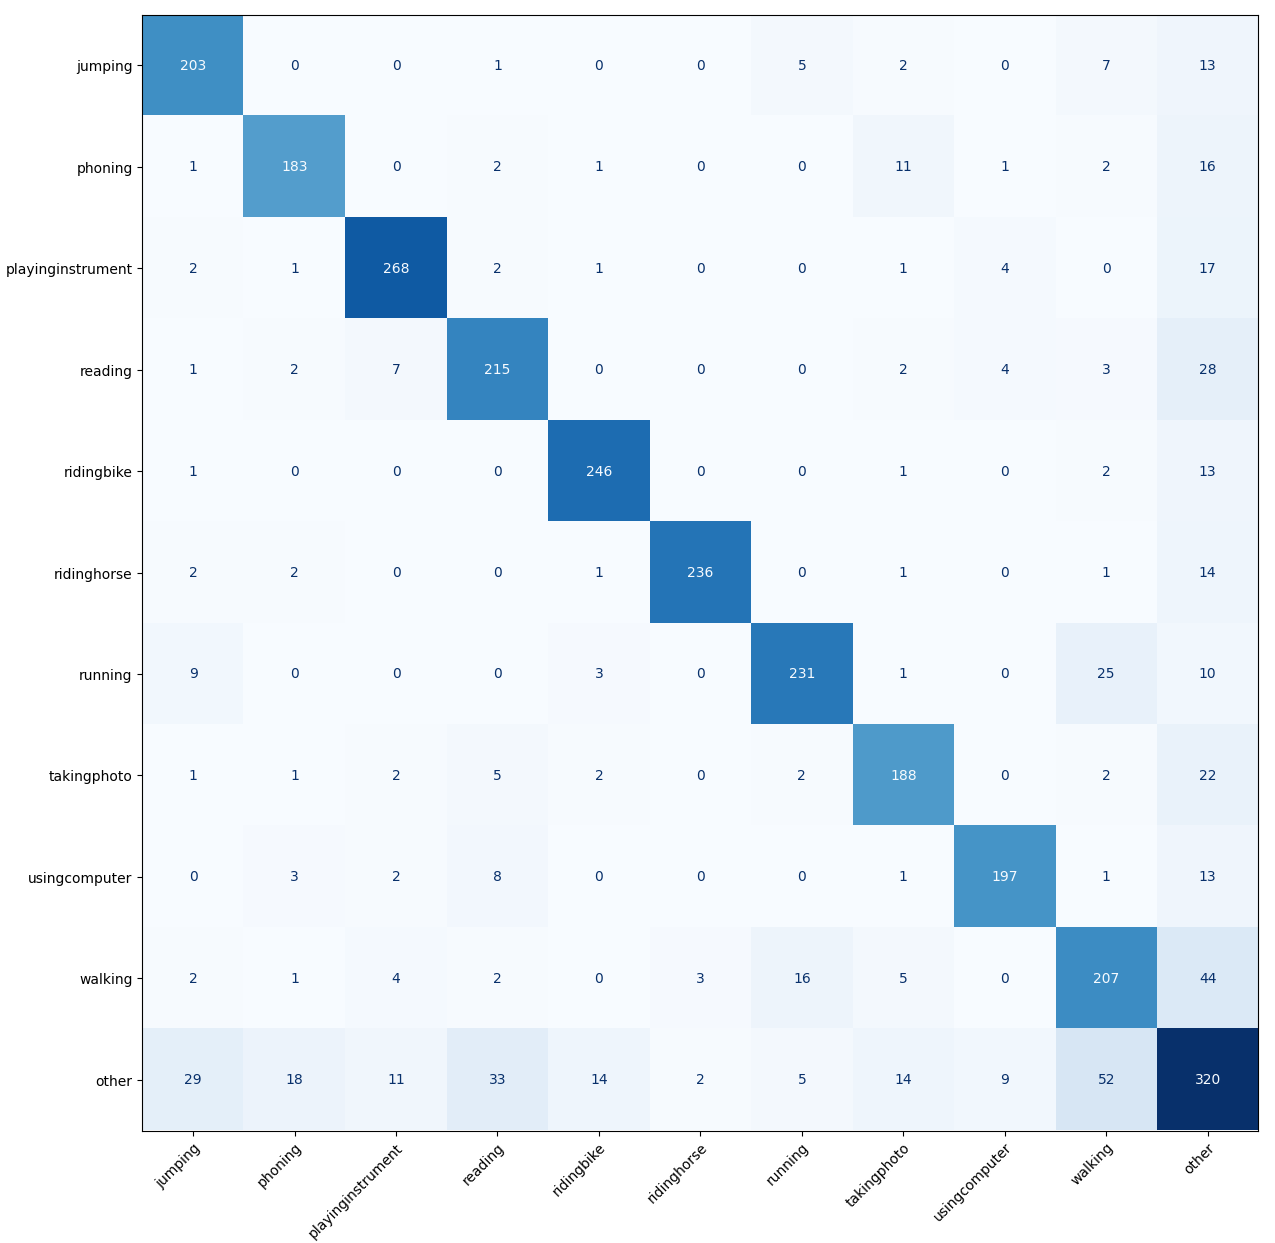
\includegraphics[width=0.66\textwidth]{confiution_matrix_voc}}
	\caption{ماتریس درهم ریختگی روش ارتباط‌سنج روی \lr{Voc 2012}}
	\label{fig: confiution_matrixvoc}
\end{figure}
\begin{figure}[ht]
	\centerline{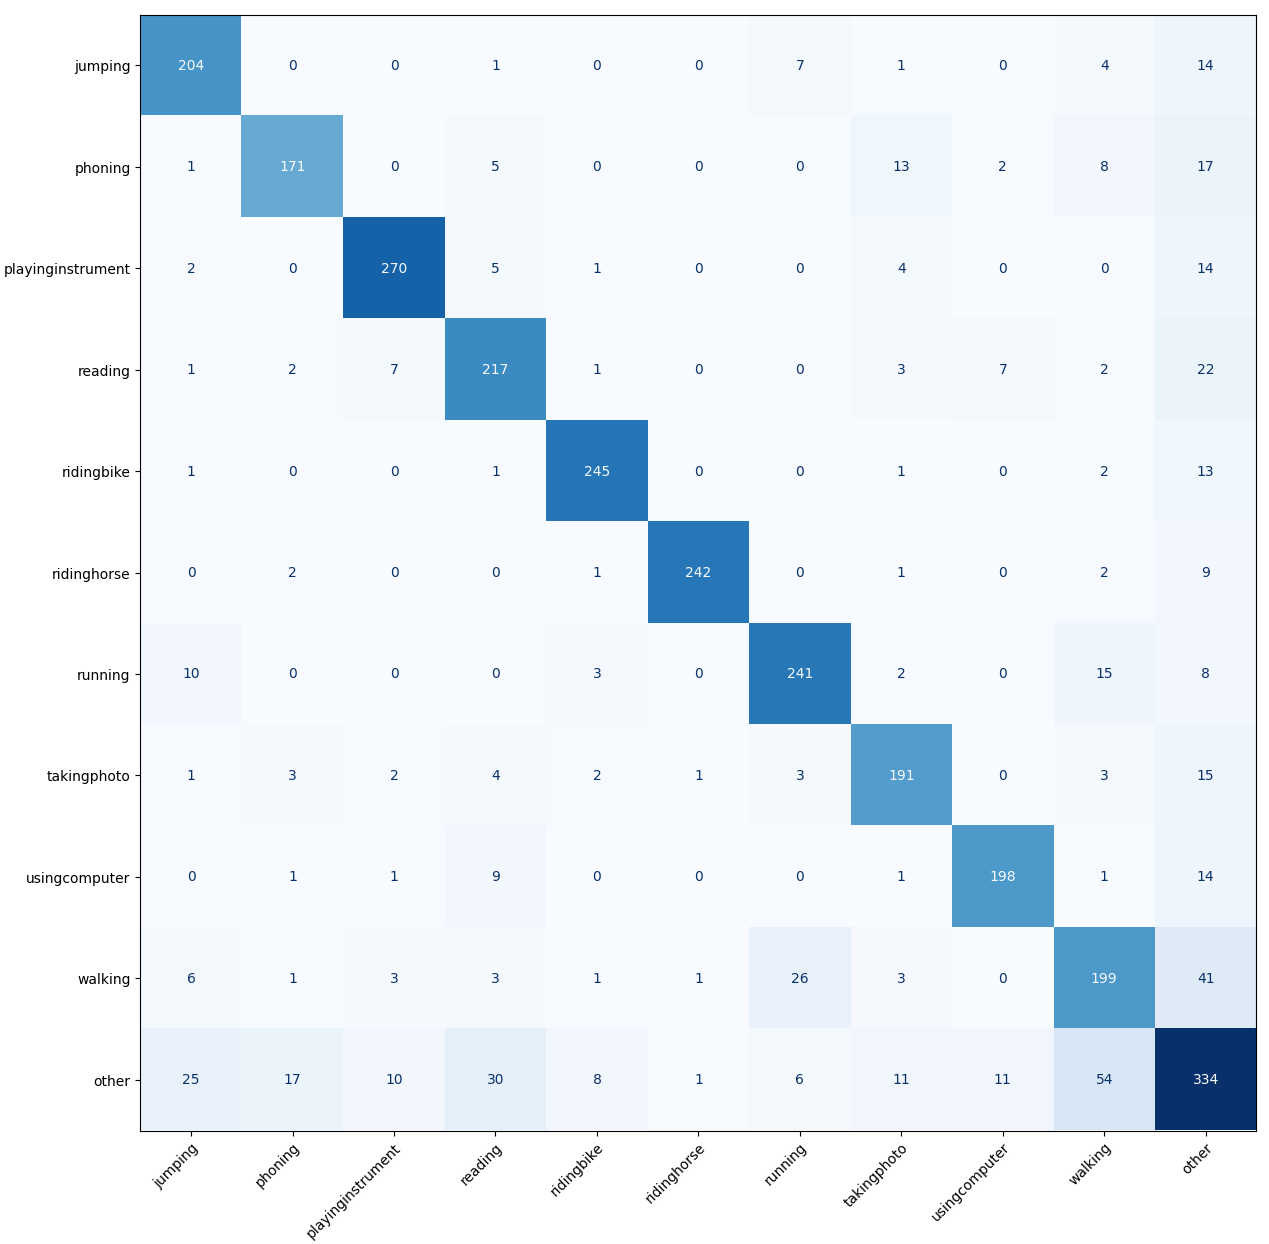
\includegraphics[width=0.66\textwidth]{confution_matrix_voc_lad}}
	\caption{ماتریس درهم ریختگی روش توصیف کننده زاویه بدن روی \lr{Voc 2012}}
	\label{fig: confution_matrix_voclad}
\end{figure}
\section{نگاه عمیق تر و تصویرسازی}\label{amig_negah}
تصاویر %
\ref{fig: confiution_matrixvoc}
از خروجی مدل در بخش %
\gls{Classifier}
قرار گرفته است. این تصاویر نشان می‌دهد که مدل به کدام بخش از ناحیه‌ی تصویر در جهت تشخیص فعالیت،‌ بیشترین توجه را دارد و بیشترین امتیاز را به کدام ناحیه اختصاص می‌دهد.
تصویر %
\ref{fig: myplot_voc}
یک نمونه تصویر از این مجموعه داده است که نشان می‌دهد 3 فعالیت در یک تصویر درحال انجام است که مدل تشخیص نقاط کلیدی بدن توانسته به صورت مجزا برای هرکدام ناحیه‌های بدن را ترسیم کند.
\begin{figure}[ht]
	\centerline{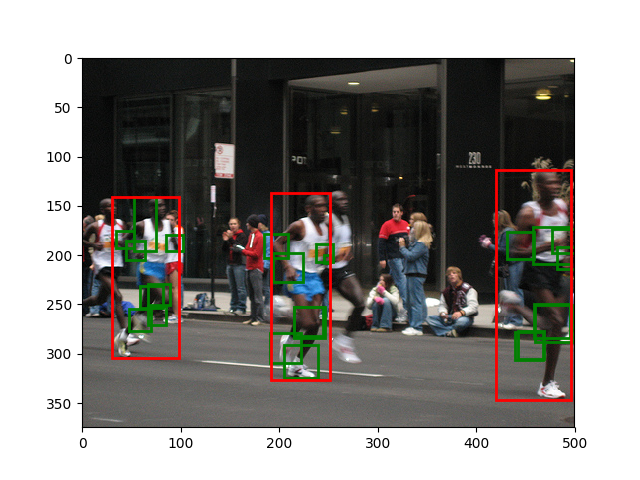
\includegraphics[width=0.8\textwidth]{myplot_voc}}
	\caption{نمونه تصویر فعالیت در \lr{Voc 2012}}
	\label{fig: myplot_voc}
\end{figure}

تصاویر %
\ref{fig:res_for_medioum images}
 از پیش‌بینی مدل در بخش ارتباط‌سنج نشان داده شده است. ناحیه سبز رنگ، ناحیه برجسته اشیاء و ناحیه آبی رنگ ناحیه برجسته اجزاء بدن را نشان می‌دهد.
   \begin{figure}
 	\centering
 	\subfloat[ ]{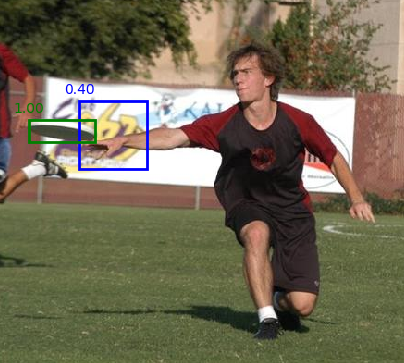
\includegraphics[width=0.24\textwidth]{res_playing}}
 	\hfill
 	\subfloat[ ]{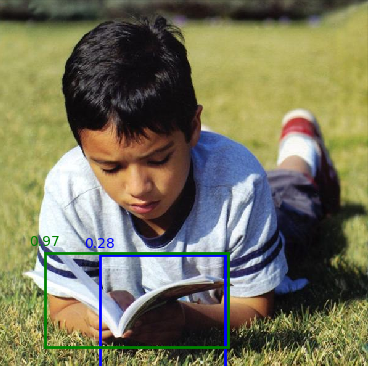
\includegraphics[width=0.24\textwidth]{res_reading}}
 	\hfill
 	\subfloat[ ]{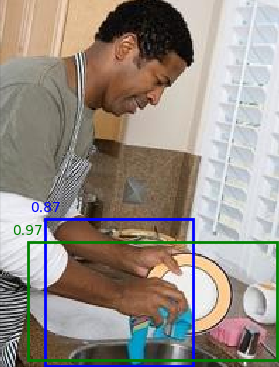
\includegraphics[width=0.24\textwidth]{res_washing_dishes}}
 	\hfill
 	\subfloat[ ]{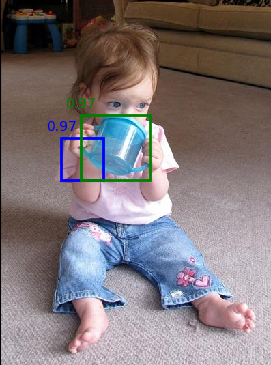
\includegraphics[width=0.24\textwidth]{res_drinking}}
 	\\
 	\subfloat[ ]{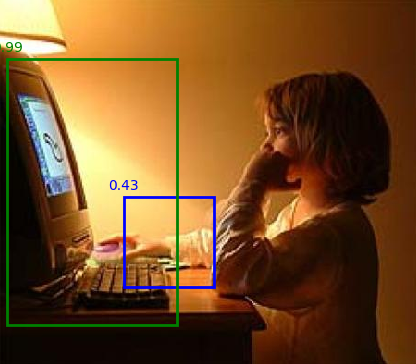
\includegraphics[width=0.24\textwidth]{res_computer}}
 	\hfill
 	\subfloat[ ]{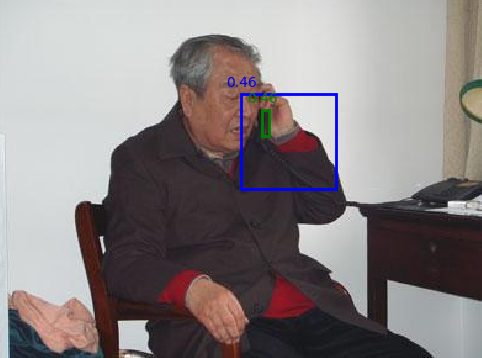
\includegraphics[width=0.24\textwidth]{res_phone_calling}}
 	\hfill
 	\subfloat[ ]{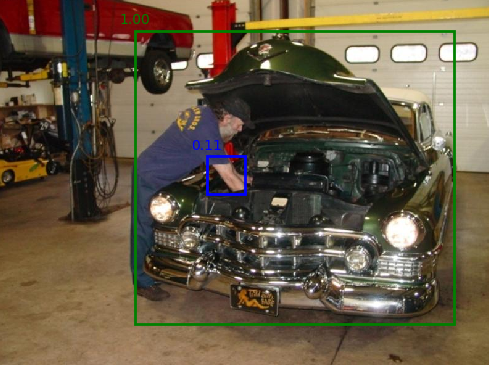
\includegraphics[width=0.24\textwidth]{res_fixing_car}}
 	\hfill
 	\subfloat[ ]{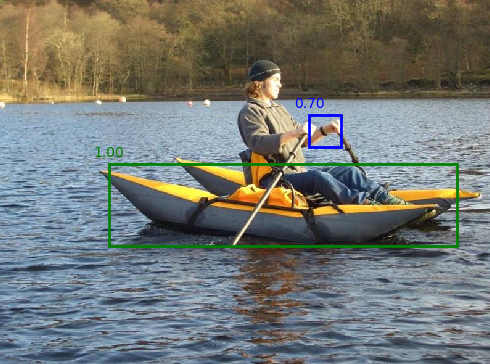
\includegraphics[width=0.24\textwidth]{res_gayeg_savari}}
 	\hfill
 	\caption{تصاویر %
 		\gls{BoundingBox}
 		 ژست بدست آمده از نقاط کلیدی}
 	\label{fig:res_for_medioum images}
 \end{figure}
همانطور که در این تصاویر مشاهده می‌شود، "دست" بیشتر عامل تاثیرگذار در تشخیص فعالیت‌هایی است که نیاز به استفاده از "دست" بیشتر است. همچنین شیء که بیشترین ارتباط را با فعالیت مورد نظر دارد نیز مشخص کرده است.

در تصاویر %
\ref{fig: confiution_matrixvoc}
یک سری از پیش‌ بینی‌های نادرست نشان داده شده است. تصاویر "آ" و "د" تقریبا باهم مشابه هستند و درهر دو دست بالا قرار گرفته است. ممکن است عاملی باشد که شبکه خروجی جا به جا تولید کرده باشد. همچنین جفت تصاویر "ب" و"ه" ظرف و شکل دست در هنگام ظرف شستن و آشپزی کردن باعث گمراهی شبکه شده و"ج" و "و" نیز به همین ترتیب. تصویر "ج" به دلیل اینکه شخص خودکار در دست گرفته است باعث شده شبکه خروجی نوشتن کتاب را پیش بینی کند.
  \begin{figure}
	\centering
	\subfloat[\color{red}تکان دادن دست
	]{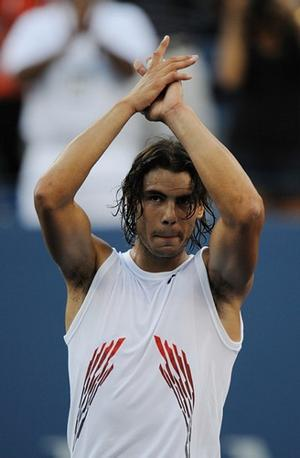
\includegraphics[width=0.25\textwidth]{applauding_216}}
	\hfill
	\subfloat[\color{red}آشپزی کردن
	]{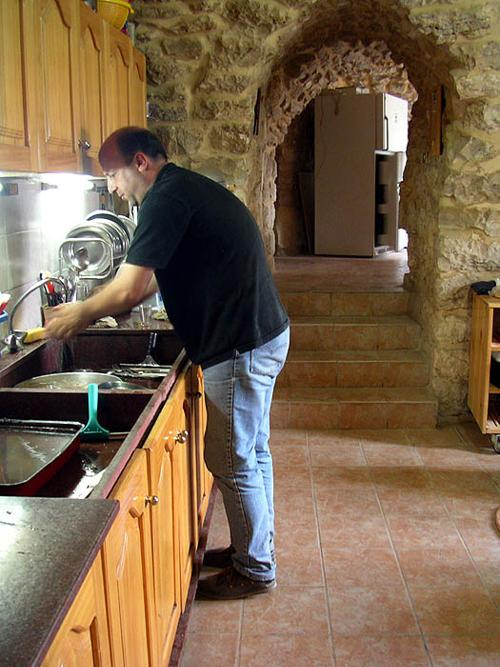
\includegraphics[width=0.25\textwidth]{washing_dishes_093}}
	\hfill
	\subfloat[\color{red}نوشتن کتاب]{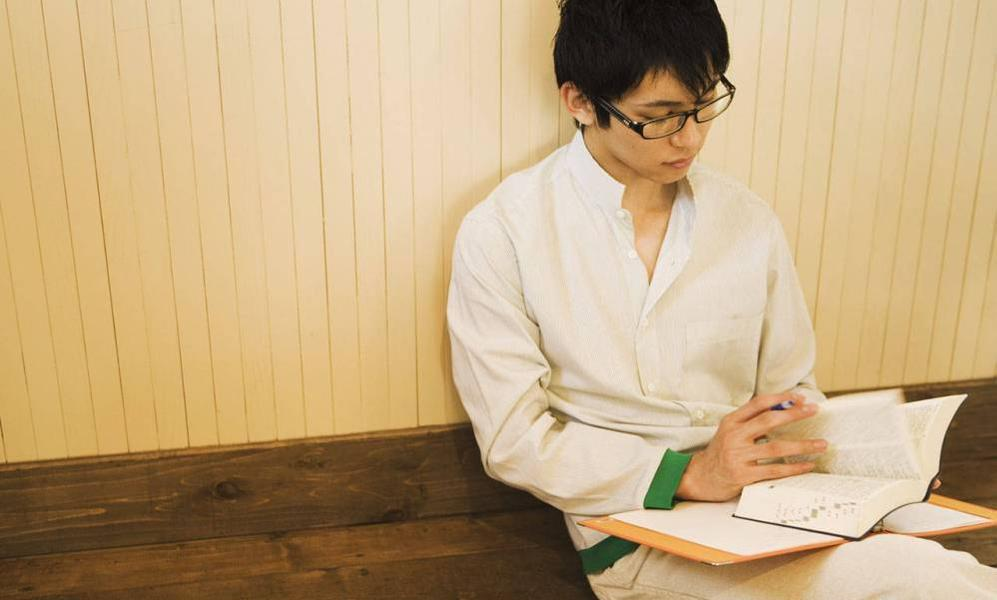
\includegraphics[width=0.30\textwidth]{reading_011}}
	\\
	\subfloat[\color{red}تشویق کردن]{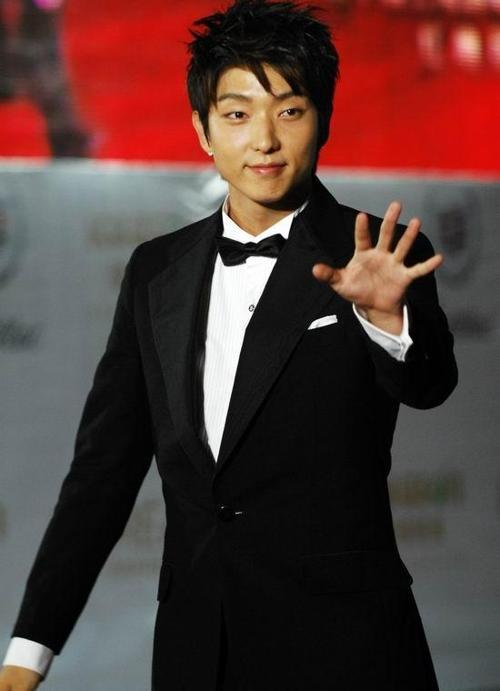
\includegraphics[width=0.25\textwidth]{waving_hands_210}}
	\hfill
	\subfloat[\color{red}ظرف شستن
	]{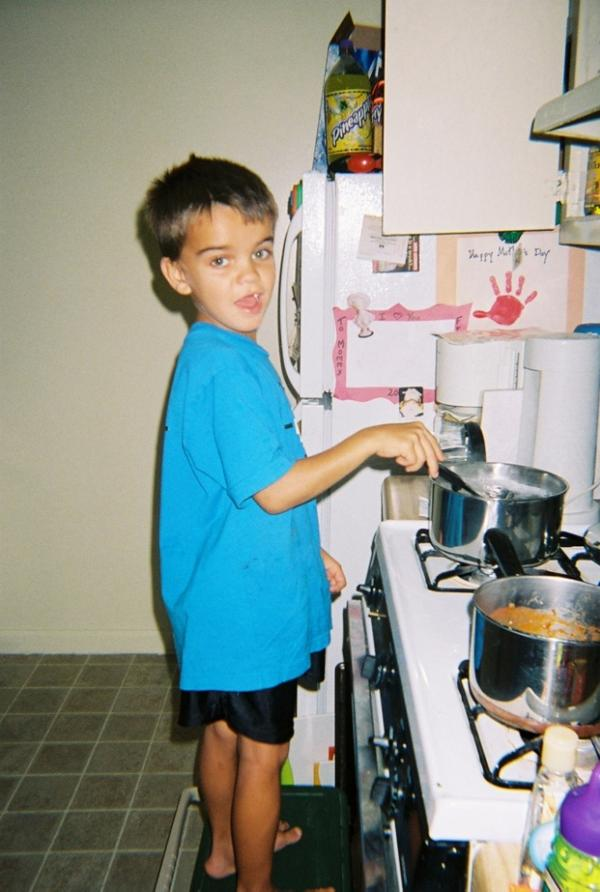
\includegraphics[width=0.25\textwidth]{cooking_006}}
	\hfill
	\subfloat[\color{red}خواندن کتاب
	]{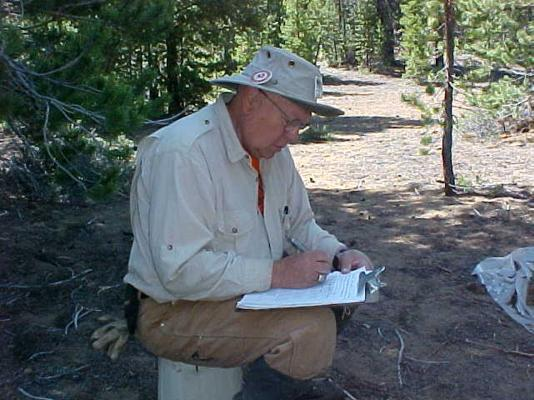
\includegraphics[width=0.30\textwidth]{writing_on_a_book_141}}
	\hfill
	\caption{تصاویری از پیش بینی‌های نادرست شبکه}
	\label{fig:res_for_false_prediction}
\end{figure}
 